%=======================================================================
%  Cloud Computing -- 100 Day Research Assignment
%  Group G18 | Section A
%  Deliverable 02: Base-Article Implementation and Real-Gap Finding
%
%  Compile:  pdfLaTeX -> BibTeX -> pdfLaTeX -> pdfLaTeX
%            (Overleaf: Menu > Compiler > pdfLaTeX; upload the whole
%             report/ folder including generated/ and figures/)
%
%  Numbers marked "Simulator" come from sim/run_all.py.
%  Numbers marked "Testbed" are filled in AUTOMATICALLY from
%  generated/tb_*.tex after you run the Kubernetes experiments and
%  python3 analysis/analyze_testbed.py. Until then they print "pending".
%=======================================================================
\documentclass[conference]{IEEEtran}
\IEEEoverridecommandlockouts

\usepackage{cite}
\usepackage{amsmath,amssymb,amsfonts}
\usepackage{graphicx}
\usepackage{booktabs}
\usepackage{array}
\usepackage{multirow}
\usepackage{url}
\usepackage[hidelinks]{hyperref}
\usepackage{xcolor}
\usepackage{tikz}
\usetikzlibrary{arrows.meta,positioning,fit,backgrounds}
\usepackage{algorithm}
\usepackage{algpseudocode}
\usepackage[section]{placeins}  % keep floats inside their section

% ---------------------------------------------------------------------
% generated numbers
% ---------------------------------------------------------------------
% generated by sim/run_all.py -- do not edit
\newcommand{\simFPrestartsMin}{1}
\newcommand{\simFPrestartsMax}{6}
\newcommand{\simFPextraShare}{47}
\newcommand{\simRseeds}{30}
\newcommand{\simOsuccnoneN}{100.0}
\newcommand{\simOsuccdpN}{99.9}
\newcommand{\simOsuccfpN}{58.9}
\newcommand{\simOsuccisoN}{100.0}
\newcommand{\simOsuccaN}{100.0}
\newcommand{\simOsuccbN}{85.5}
\newcommand{\simOsuccabN}{100.0}
\newcommand{\simOnineFPsucc}{58.9}
\newcommand{\simOnineNONEsucc}{100.0}
\newcommand{\simOnineFPrestarts}{25}
\newcommand{\simOnineFPavail}{59}
\newcommand{\simOhundredFPsucc}{13.8}
\newcommand{\simOhundredNONEsucc}{90.9}
\newcommand{\simOhundredDPsucc}{33.0}
\newcommand{\simOhundredBrestarts}{9.2}
\newcommand{\simOhundredBsucc}{68.7}
\newcommand{\simOhundredABsucc}{91.0}
\newcommand{\simOseeds}{10}
\newcommand{\simPFPpost}{4.6}
\newcommand{\simPNONEpost}{99.3}
\newcommand{\simPABpost}{99.3}
\newcommand{\simPDPrec}{29}
\newcommand{\simHFPdet}{1.5}
\newcommand{\simHAdet}{5.4}
\newcommand{\simHABdet}{5.4}
\newcommand{\simHBdet}{1.5}
\newcommand{\simDFPrestarts}{23.9}
\newcommand{\simDArestarts}{14.2}
\newcommand{\simDBrestarts}{0.8}
\newcommand{\simDABrestarts}{0.0}
\newcommand{\simDFPsucc}{66.0}
\newcommand{\simDNONEsucc}{92.2}
\newcommand{\simDABsucc}{92.2}
\newcommand{\simSharmful}{4}

% generated by experiments/local_check.py
\newcommand{\locMode}{docker --cpus=0.5}
\newcommand{\locCap}{39}
\newcommand{\locHzFifty}{1}
\newcommand{\locLzFifty}{1.1}
\newcommand{\locHzFailFifty}{0/10}
\newcommand{\locHzNinety}{1}
\newcommand{\locLzNinety}{1.1}
\newcommand{\locHzFailNinety}{0/10}
\newcommand{\locHzOneFifty}{1001}
\newcommand{\locLzOneFifty}{1.8}
\newcommand{\locHzFailOneFifty}{10/10}
\newcommand{\locHang}{5.1}

\IfFileExists{generated/tb_numbers.tex}{% generated by analysis/analyze_testbed.py -- do not edit
\makeatletter
\@namedef{tbn@cpu}{11th Gen Intel(R) Core(TM) i5-1135G7 @ 2.40GHz}
\@namedef{tbn@cpus}{8}
\@namedef{tbn@memgb}{9.6}
\@namedef{tbn@os}{Linux 6.18.33.2-microsoft-standard-WSL2 x86\_64 GNU/Linux}
\@namedef{tbn@docker}{29.9.0}
\@namedef{tb@DP@q}{7.9 $\pm$ 0.1}
\@namedef{tb@DP@s}{38.9 $\pm$ 0.1}
\@namedef{tb@DP@succ}{6824}
\@namedef{tb@DP@rs}{1.0 $\pm$ 0.0}
\@namedef{tb@DP@ready}{72}
\@namedef{tb@DP@n}{3}
\@namedef{tb@DP@catcpu}{96}
\@namedef{tb@DP@catmib}{2.6}
\@namedef{tb@DP@skicpu}{--}
\@namedef{tb@DP@skimib}{--}
\@namedef{tb@DP@warm}{0.0}
\@namedef{tb@FP@q}{0.1 $\pm$ 0.1}
\@namedef{tb@FP@s}{2.5 $\pm$ 0.4}
\@namedef{tb@FP@succ}{28595}
\@namedef{tb@FP@rs}{1.0 $\pm$ 0.0}
\@namedef{tb@FP@ready}{288}
\@namedef{tb@FP@n}{3}
\@namedef{tb@FP@catcpu}{103}
\@namedef{tb@FP@catmib}{2.4}
\@namedef{tb@FP@skicpu}{--}
\@namedef{tb@FP@skimib}{--}
\@namedef{tb@FP@warm}{0.0}
\@namedef{tb@SKI@q}{0.1 $\pm$ 0.0}
\@namedef{tb@SKI@s}{2.1 $\pm$ 0.1}
\@namedef{tb@SKI@succ}{28435}
\@namedef{tb@SKI@rs}{1.0 $\pm$ 0.0}
\@namedef{tb@SKI@ready}{286}
\@namedef{tb@SKI@n}{3}
\@namedef{tb@SKI@catcpu}{107}
\@namedef{tb@SKI@catmib}{2.0}
\@namedef{tb@SKI@skicpu}{12}
\@namedef{tb@SKI@skimib}{6.2}
\@namedef{tb@SKI@warm}{0.0}
\@namedef{tbn@Rdone}{1}
\@namedef{tbn@cap}{10.8}
\@namedef{tbn@Cdone}{1}
\@namedef{tbn@Odone}{1}
\@namedef{tbn@Oruns}{7}
\@namedef{tbn@Pdone}{1}
\@namedef{tbn@Pruns}{7}
\@namedef{tbn@Hdone}{1}
\@namedef{tbn@Hruns}{12}
\@namedef{tbn@Ddone}{1}
\@namedef{tbn@Druns}{12}
\@namedef{tbn@Oloads}{90\,\%}
\@namedef{tbn@ablationdone}{1}
\@namedef{tbn@govcpu}{2.00}
\@namedef{tbn@govmib}{9.3}
\@namedef{tbn@Pfig}{1}
\@namedef{tbn@Dfig}{1}
\makeatother
}{}
\makeatletter
% \TB{arm}{metric}: testbed value or "pending"
\newcommand{\TB}[2]{\@ifundefined{tb@#1@#2}{\textit{pending}}{\@nameuse{tb@#1@#2}}}
% \TBN{name}: testbed number or "pending"
\newcommand{\TBN}[1]{\@ifundefined{tbn@#1}{\textit{pending}}{\@nameuse{tbn@#1}}}
% \IfTB{name}{if-run}{if-not-run}
\newcommand{\IfTB}[3]{\@ifundefined{tbn@#1}{#3}{#2}}
% \tabinput{file}: \input that is safe inside tabular (primitive input)
\newcommand{\tabinput}[1]{\@@input #1 }
\makeatother

% testbed table rows: real rows if the file exists, else a "pending" row
\newcommand{\deftbrows}[2]{\IfFileExists{generated/tb_table_#1.tex}%
  {\expandafter\def\csname tbrows#1\endcsname{\tabinput{generated/tb_table_#1.tex}}}%
  {\expandafter\def\csname tbrows#1\endcsname{\pending{#2}\\}}}
\newcommand{\tbrows}[1]{\csname tbrows#1\endcsname}
\newcommand{\pending}[1]{\multicolumn{#1}{c}{\textit{pending -- run the testbed scripts (Appendix~\ref{app:run})}}}
\deftbrows{P}{5}\deftbrows{H}{5}\deftbrows{D}{5}\deftbrows{ablation}{9}
\newcommand{\gapbox}[1]{%
  \begin{center}
  \fbox{\begin{minipage}{0.95\columnwidth}\small #1\end{minipage}}
  \end{center}}
\newcommand{\FPA}{FP+A}
\newcommand{\FPB}{FP+B}
\newcommand{\FPAB}{FP+A+B}

\begin{document}

\title{When Self-Healing Hurts:\\ Reproducing Signal-Based Health Monitoring for\\
Kubernetes and Fixing Probe-Induced Restart Cascades\\[2pt]
\large Deliverable 02 -- Base-Article Implementation and Real-Gap Finding}

\author{
\IEEEauthorblockN{M. Yasir Suhail}
\IEEEauthorblockA{\textit{Department of Computer Science}\\
\textit{FAST-NUCES, Islamabad}\\
Section A, Group G18}
\and
\IEEEauthorblockN{M. Aashir Sheraz}
\IEEEauthorblockA{\textit{Department of Computer Science}\\
\textit{FAST-NUCES, Islamabad}\\
Section A, Group G18}
}

\maketitle

%======================================================================
\begin{abstract}
Kubernetes restarts a container when its liveness probe fails. Our base
paper, Roberts \emph{et al.}~\cite{roberts2025}, shows that this
poll-based monitoring is slow and proposes signal-based monitoring
(SKI) instead. In this deliverable we (1)~re-implement the core of that
paper on stock Kubernetes, without the authors' modified kubelet, and
reproduce its main results; (2)~use the reproduction to locate a real
gap: the paper tests one pod under light load, a setting in which a
probe can never cause a cascade, and neither probes nor SKI look at all
replicas together before restarting; (3)~propose a method with two
parts: \emph{progress-based liveness} (A), which judges a container by
whether it still finishes work rather than by whether it answers
quickly, and a \emph{cluster-aware restart governor} (B), which holds
restarts back when many replicas fail at the same time; and (4)~evaluate
it with an ablation. A calibrated simulator reproduces the paper's
detection times within about 1\,s. It shows that at 90\,\% load the
paper's ``fast probe'' baseline cuts successful requests from
\simOnineNONEsucc\,\% to \simOnineFPsucc\,\% even though nothing is
broken. After a 60\,s load spike it leaves the service at
\simPFPpost\,\% success; with no probe at all the service recovers to
\simPNONEpost\,\%. A+B removes all of these false restarts, keeps
\simDABsucc\,\% success during a dependency stall
(baseline: \simDFPsucc\,\%), and still detects a silently hung
replica within \simHABdet\,s. All code, scripts and a one-command
Kubernetes testbed for an 8\,GB laptop are provided. Testbed tables in
this report fill in automatically from the raw runs.
\end{abstract}

\begin{IEEEkeywords}
Kubernetes, liveness probe, self-healing, failure detection, overload,
restart cascade, metastable failure, reproducibility
\end{IEEEkeywords}

%======================================================================
\section{Introduction}
%======================================================================
Self-healing is one of the main reasons people run services on
Kubernetes. The kubelet sends a \emph{liveness probe} (an HTTP request,
TCP connect or command) to each container every few seconds. If the
container fails a number of probes in a row, the kubelet kills and
restarts it~\cite{k8sprobes}. The hidden assumption is simple:
\emph{a container that does not answer in time is broken.}

In Cutoff~1 we argued that this assumption is wrong under overload. A
busy container is slow, not broken. If its health endpoint waits in the
same queue as real requests, the probe times out and the healthy
container is killed. Its traffic moves to the other replicas, which then
slow down and fail their probes too. The repair mechanism becomes the
fault.

This deliverable follows the workflow the instructor asked for. We
\emph{reproduce} the base paper, \emph{analyse} it, find a
\emph{defensible gap}, then \emph{design, implement and evaluate} our own
method with an ablation study. Our contributions are:

\begin{enumerate}
\item \textbf{A decision and a reproducibility check} for the base paper
  (Sec.~\ref{sec:selection}). We keep Roberts \emph{et al.} and
  explain why, including what is missing from it.
\item \textbf{A working re-implementation of its core method on stock
  Kubernetes} (Sec.~\ref{sec:repro}). The paper's SKI needs a modified
  kubelet that is not public. We rebuild the same signal path with a log
  sidecar, a shared PID namespace and a readiness gate. We also give a
  calibrated simulator that reproduces the paper's Tables~IV--VI.
\item \textbf{An explanation for the paper's own unexplained result.}
  The extra ``fast probe'' restarts come from a race between start-up
  and the first liveness probe (Sec.~\ref{sec:fpexplain}).
\item \textbf{A defensible research gap}, shown with evidence: the
  cascade appears only when there is more than one replica, which the
  paper never tests (Sec.~\ref{sec:gap}).
\item \textbf{A proposed method} (progress-based liveness + cluster-aware
  restart governor), its code, and an \textbf{ablation} over four fault
  and load scenarios (Secs.~\ref{sec:method}--\ref{sec:results}).
\end{enumerate}

%======================================================================
\section{Selecting the Base Paper: Does It Fit?}
\label{sec:selection}
%======================================================================
\subsection{The selected paper}
\begin{itemize}
\item \textbf{Title:} Signalling Health for Improved Kubernetes
  Microservice Availability~\cite{roberts2025}
\item \textbf{Authors:} Jacob Roberts, Blair Archibald, Phil Trinder
  (University of Glasgow)
\item \textbf{Venue / year:} arXiv preprint 2507.02158 (cs.DC), July 2025
\item \textbf{Paper link:} \url{https://arxiv.org/abs/2507.02158}
\item \textbf{GitHub / project link:} none published. The paper links
  only to SockShop~\cite{sockshop}, Locust~\cite{locust}, Kubernetes and
  CRI-O.
\end{itemize}

\subsection{Reproducibility check}
Table~\ref{tab:repro-check} goes through the instructor's checklist. The
paper is weak on released artefacts. Its \emph{core method}, however, is
small and fully specified. It consists of four probe settings
(Table~II of the paper), a closed-form detection-time model, one public
benchmark service, one load generator and one fault at a fixed time.
That is exactly the ``core methodology'' the instructor asks us to
implement.

\begin{table}[t]
\centering
\caption{Reproducibility check of the base paper}
\label{tab:repro-check}
\footnotesize
\begin{tabular}{@{}p{2.3cm}p{1.1cm}p{4.1cm}@{}}
\toprule
Item & Available & What we did \\
\midrule
Official repository & No & Re-implemented everything (Go + YAML) \\
Source code (SKI) & No & Built an SKI emulation on stock K8s \\
Modified kubelet & No & Not needed: sidecar + PID ns + readiness gate \\
Experiment scripts & No & Wrote \texttt{experiments/*.sh} \\
Benchmark / data & Yes & SockShop catalogue + catalogue-db images \\
Configuration & Partly & Probe table given; \texttt{timeoutSeconds} and startup-probe values missing \\
Software versions & Yes & K8s 1.27.8, CRI-O 1.27.1; we use K8s 1.27.13 (kind) \\
Hardware & Yes & 1 VM, 8 vCPU, 32\,GB; we use a laptop \\
Install / run guide & No & \texttt{docs/GUIDE.md} \\
Reported results & Yes & Tables III--VI used as targets \\
\bottomrule
\end{tabular}
\end{table}

\subsection{Alternatives considered}
We looked for a better-documented base paper in the same area before
deciding. Flora \emph{et al.}~\cite{flora2022} study probe
\emph{false negatives} under software ageing. They publish no code, and
their topic is the opposite failure mode to ours. Chen
\emph{et al.}~\cite{chen2025} inject node, pod and network faults at
scale, but they do not study probes and release no code. Vayghan
\emph{et al.}~\cite{vayghan2019} treat Kubernetes as an availability
manager, but their work is older, uses no probes under load and has no
public artefact. None of these is easier to reproduce, and none of them
touches our research question.

\textbf{Decision.} We keep Roberts \emph{et al.} for three reasons.
\begin{itemize}
\item It is the closest work to our question.
\item It \emph{observes} the very phenomenon we study but cannot explain
  it.
\item Its future-work section predicts our result: ``we expect PCM to
  erroneously detect high network latency as container failure''.
\end{itemize}
Its two weaknesses are that it is a preprint and that it has no code. We
handle both openly by publishing a full re-implementation.

\subsection{A note on ``datasets'' and modality}
This is a \emph{systems} paper, not a machine-learning paper. There is
no training data and no text, image or audio modality. The equivalent of
a dataset is the \emph{benchmark service plus the workload}.
Section~\ref{sec:data} documents these the way the instructor asked for
datasets.

%======================================================================
\section{Understanding the Base Paper}
\label{sec:understand}
%======================================================================
\textbf{Problem.} Kubernetes notices failures by \emph{polling}
(poll-based container monitoring, PCM). Polling must be tuned by hand.
Detection takes several probe periods. Badly tuned probes can lower
availability.

\textbf{Why it matters.} Every second between a failure and its repair
is lost availability. Default probe settings in benchmarks such as
SockShop take minutes to recover a pod.

\textbf{Proposed solution.} In \emph{signal-based} monitoring (SCM), the
container \emph{tells} the orchestrator when its state changes. In SKI,
the Kubernetes prototype, a sidecar follows the container's log through
the API server. A matching log line makes the sidecar notify a
\emph{modified kubelet} over a UNIX socket. The kubelet then marks the
container Ready or restarts it at once.

\textbf{Analytical model.} Detection time for polling is
$T_{l,p}\approx (N_l-\tfrac12)I_l+L_l$, where $N_l$ is the failure
threshold, $I_l$ the period and $L_l$ the probe latency. For signals
it is $T_{l,s}\approx L_s$.

\textbf{Cloud component.} Self-healing in a container orchestrator: the
kubelet's monitor--decide--act loop on each node.

\textbf{Benchmark and baselines.} SockShop's \texttt{catalogue} service
(one pod) backed by \texttt{catalogue-db}. The two baselines are the
SockShop default probes (DP: 3 failures, every 3\,s, delays 300/180\,s)
and fast probes (FP: 1 failure, every 1\,s, delay 1\,s).

\textbf{Metrics.} Time to queue a restart, time to start the restart,
total/failed/HTTP-500 requests, cumulative Ready pods, CPU and memory
overhead.

\textbf{Settings.} One VM (8 vCPU, 32\,GB), single-node Kubernetes
1.27.8, CRI-O 1.27.1, one pod per service, Locust at $\le$100\,req/s
with a 0.5\,s timeout, a 6-minute warm-up, failure at 60\,s, 290\,s
windows and 30 runs per configuration.

\textbf{Assumptions.} Failures are clean (a process dies) and the
container can \emph{say} it failed by writing a log line. There is only
one replica.

\textbf{Limitations the authors state.} A simple failure model, a small
benchmark and a single node with one pod. SKI does not aggregate status
across pods. Its log fetching may not scale. ``It remains unclear why
most restarts under FP occur after the failure at 60\,s.''

\textbf{Missing or unclear details.} No code. No \texttt{timeoutSeconds}
or startup-probe values. Locust user count, spawn rate and wait time
are not given, and neither are the log patterns SKI matches. The
``catalogue bug'' adds restarts that are not part of the experiment.

%======================================================================
\section{Benchmark, Workloads and Data}
\label{sec:data}
%======================================================================
Table~\ref{tab:data} lists every workload used, in the format the
instructor asked for. Nothing is ``trained'', so there is no
train/validation/test split. Instead, every configuration is
\emph{repeated} with different random seeds. Simulator runs are fully
seeded and therefore exactly repeatable.

\begin{table*}[t]
\centering
\caption{Workloads (the ``datasets'' of this systems study)}
\label{tab:data}
\footnotesize
\begin{tabular}{@{}p{2.9cm}p{2.1cm}p{2.6cm}p{4.6cm}p{4.6cm}@{}}
\toprule
Name & Source & Size & Characteristics & Pre-processing / use \\
\midrule
SockShop \texttt{catalogue} 0.3.5 + \texttt{catalogue-db} 0.3.0 &
Docker Hub, \cite{sockshop} & 2 images, 9 catalogue items (MySQL) &
Go REST service; \texttt{/health} pings the DB; Ready in $\approx$2\,s after start &
Unchanged image; run under a shell wrapper exactly as the paper does (liveness test) \\
Paper workload (R) & Re-created from \cite{roberts2025} & 100 users $\times$ 1 req/s, 290\,s & Closed model, 0.5\,s timeout, \texttt{GET /catalogue} & Our Go generator in \emph{closed} mode replaces Locust \\
G18 service under test & This work (\texttt{src/cmd/sut}) & 6 replicas, 4 workers each & CPU-bound \texttt{/work} behind a FIFO pool shared with \texttt{/healthz} & CPU limit 200m; fixed CPU work per request \\
Overload workloads (O, P) & This work & 60--120\,\% of measured capacity, 240\,s & Open model, Poisson arrivals, 2\,s timeout; P = 70\,\%$\rightarrow$150\,\% spike for 60\,s & Rates scaled by the calibrated capacity (Exp.~C) \\
Fault workloads (H, D) & This work & 70\,\% load, 240\,s & H: one replica hangs silently at 60\,s; D: shared dependency stalls 20\,s & Faults injected through admin endpoints \\
Raw results & Generated & $\approx$300\,KB per run & Per-second request counts, 1\,Hz pod state, events, logs & \texttt{analysis/analyze\_testbed.py} \\
\bottomrule
\end{tabular}
\end{table*}

%======================================================================
\section{Reproduction Setup}
\label{sec:repro}
%======================================================================
\subsection{Two complementary instruments}
We reproduce the paper in two ways.

\textbf{(1) Kubernetes testbed} (\texttt{experiments/}). This is a kind
cluster~\cite{kind} pinned to Kubernetes 1.27.13, the closest 1.27
release that kind ships. It runs on one laptop, with the same
single-node, single-pod design as the paper. Each run gets its own
namespace, so events from one run cannot leak into the next. Load comes
from a generator \emph{inside} the cluster, so it goes through the
normal Service load balancing.

\textbf{(2) Discrete-event simulator} (\texttt{sim/probesim.py}, about
900 lines of Python). It models the same mechanisms one by one:
\begin{itemize}
\item a FIFO worker pool and a CPU limit;
\item kubelet probe workers;
\item the kubelet restart back-off, as coded in Kubernetes~1.27
  (\texttt{doBackOff});
\item endpoint propagation;
\item open and closed clients;
\item the faults;
\item both proposed components.
\end{itemize}
The simulator lets us run thousands of seeded runs in minutes and sweep
settings a laptop cannot sweep. The testbed checks that the effects are
real.

\subsection{SKI on stock Kubernetes}
Table~\ref{tab:ski} maps each part of SKI to our emulation. The signal
path is the same: the sidecar follows the log, matches a pattern and
acts. Only the last step differs, because we may not modify the kubelet.

\begin{table}[t]
\centering
\caption{SKI (paper) vs.\ our emulation}
\label{tab:ski}
\footnotesize
\begin{tabular}{@{}p{3.3cm}p{4.3cm}@{}}
\toprule
Paper (modified kubelet) & Ours (stock Kubernetes 1.27) \\
\midrule
Sidecar follows log via API & Same (\texttt{src/cmd/ski}) \\
Substring match & Same (\texttt{G18-FAILURE}, \texttt{transport=HTTP}) \\
Kubelet queues restart & SIGKILL via shared PID namespace; kubelet restarts container \\
2\,s termination grace & 2\,s delay before the kill \\
Kubelet marks Ready & Sidecar sets a readiness-gate condition~\cite{k8sreadinessgate} \\
\bottomrule
\end{tabular}
\end{table}

\subsection{Environment}
\textbf{Hardware.} The paper used a VM with 8 vCPU and 32\,GB. Our target
is an HP 348 laptop (Intel Core i5, 4 cores/8 threads, 8\,GB). The
testbed records the machine it actually ran on in
\texttt{results/testbed/environment.txt}. For the run used here: CPU
\TBN{cpu}, \TBN{cpus} threads, \TBN{memgb}\,GB RAM, OS \TBN{os},
Docker \TBN{docker}.

\textbf{Cloud resources.} None. The study is designed to run on one
laptop. CPU limits make each pod saturate before the machine does.

\textbf{Software.} Kubernetes 1.27.13 (kind v0.23.0, containerd), Go
1.22, Python 3.10+ with matplotlib. The simulator and analysis need no
other packages.

\textbf{Key settings} are kept in \texttt{experiments/config.env}. They
include 100 users at 1\,req/s with a 0.5\,s timeout, failure at 60\,s, a
290\,s window, the paper's probe table, 6 replicas, 4 workers, a 200m
CPU limit and stall window $W=5$\,s.

\subsection{Deviations from the original experiment}
\begin{enumerate}
\item \textbf{containerd instead of CRI-O, and K8s 1.27.13 instead of
  1.27.8.} The probe and restart code paths are the same.
\item \textbf{Locust is replaced by our Go generator in closed mode.}
  The generator is lighter and is not needed on the host. The paper does
  not give its Locust settings.
\item \textbf{Shorter warm-up for FP and SKI} (120\,s instead of 360\,s).
  Liveness starts after 1\,s, so the warm-up only has to let the pod
  settle. DP keeps 330\,s because its liveness delay is 300\,s.
\item \textbf{No ``catalogue bug''.} The database is started first and
  shared, so the start-up restart the paper describes does not happen.
  The expected number of restarts is therefore 1 rather than 2.
\item \textbf{Fewer repetitions} on the testbed: 3 runs per
  configuration (``quick'' profile) or 5 (``full''), not 30. The
  simulator uses 30.
\end{enumerate}

%======================================================================
\section{Reproduction Results}
\label{sec:reproresults}
%======================================================================
Table~\ref{tab:repro} puts the paper, the simulator and the testbed side
by side.

\begin{table*}[t]
\centering
\caption{Reproduction of Roberts et al.\ (Tables IV--VI of the paper).
Mean $\pm$ std. Simulator: \simRseeds{} seeded runs per arm. Testbed:
\TB{FP}{n} runs per arm on the laptop.}
\label{tab:repro}
\footnotesize
\begin{tabular}{@{}llccc@{}}
\toprule
Arm & Metric & Original paper & Reproduced (simulator) & Reproduced (testbed) \\
\midrule
\tabinput{generated/sim_table_R.tex}
\bottomrule
\end{tabular}

\vspace{2pt}
\raggedright\footnotesize
$^\dagger$The paper expects 2 restarts under FP: one from its start-up
``catalogue bug'' and one from the failure. It observes 3$\pm$1 (range
2--6). Our setup has no start-up bug, so we expect 1.
``Successful requests'' $=$ total $-$ failed in the paper's Table~V. We
compare successes because the paper's Locust users stop sending while
the service is down, so its \emph{total} counts are not comparable
(Sec.~\ref{sec:diff}).
\end{table*}

\begin{figure}[t]
\centering
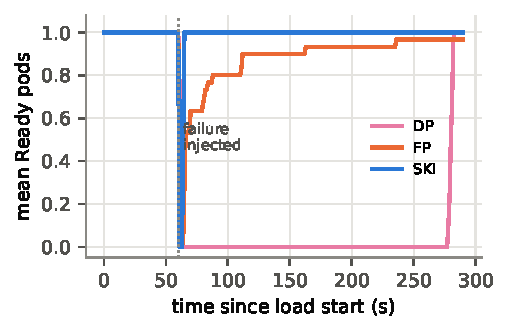
\includegraphics[width=\columnwidth]{figures/sim_R_ready.pdf}
\caption{Mean number of Ready catalogue pods (simulator, 30 runs). This
is the counterpart of the paper's Fig.~7. DP needs 180\,s of readiness
delay after the restart. FP sometimes enters a restart loop. SKI recovers
in about 2\,s.}
\label{fig:rready}
\end{figure}

\subsection{What was reproduced}
\textbf{Detection times.} The simulator gets within about 1\,s of every
detection time in the paper:
\begin{itemize}
\item DP: 7.9\,s vs.\ 8.7\,s to queue, 38.1\,s vs.\ 38.9\,s to start;
\item FP: 0.8\,s vs.\ 0.7\,s to queue, 3.0\,s vs.\ 2.9\,s to start;
\item SKI: 0.1\,s vs.\ 0.1\,s to queue, 2.3\,s vs.\ 2.2\,s to start.
\end{itemize}

\textbf{Successful requests.} The counts match closely: 6902 vs.\ 6890
(DP), 25\,961 vs.\ 26\,900 (FP) and 28\,506 vs.\ 27\,989 (SKI).

\textbf{Availability.} Cumulative Ready pods are 73/263/288 against the
paper's 80/274/286. The ranking DP $\ll$ FP $<$ SKI and the ``3.4--3.6
times better than DP'' result both hold.

\subsection{Explaining the paper's unexplained FP restarts}
\label{sec:fpexplain}
The paper reports 3$\pm$1 restarts under FP (up to 6) and states that
``it remains unclear why most restarts under FP occur after the failure
at 60\,s.'' Our model gives an explanation.

FP starts liveness probing 1\,s after the container starts, with a
threshold of 1. The catalogue needs about 1.5\,s to start listening. The
first probe after a restart therefore often lands \emph{before} the
service is up. It fails, and the new container is killed again.

The kubelet's back-off makes the first two such restarts free. From the
third restart it adds 10\,s, then 20\,s, and so on. This also explains
the paper's remark that back-off ``was applied inconsistently''. With
this one mechanism the simulator produces \simFPrestartsMin--\simFPrestartsMax{}
restarts after the failure (mean 1.9 over an expected 1). Extra restarts
occur in \simFPextraShare\,\% of runs, and almost all of them come right
after the induced failure, just as the paper observed.

On the testbed this can be checked directly. The kubelet events for
these restarts read ``Liveness probe failed: \ldots connection
refused'', and they appear within 2\,s of a container start.

\subsection{Differences and possible reasons}
\label{sec:diff}
\begin{enumerate}
\item \textbf{Total and failed request counts.} The paper's DP arm sends
  only 7600 of the 29\,000 possible requests. Its Locust users therefore
  \emph{block} while no endpoint exists, instead of failing fast. Our
  generator fails fast, so we count those requests as failed.
  \emph{Successful} requests are the comparable quantity, and they
  match.
\item \textbf{DP queue time: 7.9 vs.\ 8.7\,s.} The paper's own model
  also predicts about 7.7\,s. The authors attribute the extra second to
  failure timing inside the probe period. We see the same gap, which
  points to kubelet scheduling slack that neither model includes.
\item \textbf{FP availability: 263 vs.\ 274.} This depends strongly on
  the catalogue start-up time and on back-off timing. We calibrated the
  start-up time to the paper's ``Ready in about 2\,s''. A slightly faster
  start gives fewer restart loops.
\item \textbf{Hardware and runtime.} A laptop instead of an 8 vCPU VM,
  and containerd instead of CRI-O, change start-up and exec latencies
  by tens to hundreds of milliseconds.
\end{enumerate}

\subsection{Overhead (paper's Exp.~1)}
The paper reports that SKI adds 0.04 vCPU and 9\,MiB per pod. On the
testbed we read cgroup counters during the first 55\,s of load:
\begin{itemize}
\item catalogue alone: \TB{FP}{catcpu} millicores, \TB{FP}{catmib}\,MiB;
\item SKI sidecar: \TB{SKI}{skicpu} millicores, \TB{SKI}{skimib}\,MiB.
\end{itemize}

%======================================================================
\section{Problems Encountered}
\label{sec:problems}
%======================================================================
\textbf{Missing resources.} The paper releases no code and no modified
kubelet, and leaves the timeout and startup-probe values undocumented
(Sec.~\ref{sec:selection}).

\textbf{Installation.} The paper's own environment cannot be installed,
because the modified kubelet is private. Docker Hub rate limits can stop
\texttt{kind} pulls, so the setup script pre-loads every image into the
node once. The catalogue cannot bind port~80 as a non-root user without
extra capabilities, so we use its own default port, 8080.

\textbf{Code problems found in our Cutoff-1 code.} Our review found
three bugs. Each would have invalidated the study:
\begin{enumerate}
\item \texttt{kubectl port-forward svc/sut} tunnels \emph{all} traffic
  to \emph{one} pod. The other five replicas got no load, so load
  redistribution, the mechanism we study, could not happen. The
  forward also died whenever that pod restarted. \emph{Fix:} an
  in-cluster load generator.
\item \texttt{burn()} looped until a \emph{wall-clock} deadline. A
  throttled container therefore did \emph{less} work rather than taking
  longer, and the 200m CPU limit never limited capacity. \emph{Fix:} a
  fixed amount of CPU work per request.
\item Restart attribution read \emph{all} \texttt{Unhealthy} events,
  which mixes readiness and liveness failures. Events from earlier runs
  in the same namespace leaked into later ones. \emph{Fix:} one
  namespace per run, and only events reading ``failed liveness probe,
  will be restarted'' are counted.
\end{enumerate}

\textbf{Computational limits.} A laptop cannot run 30 repetitions of
every arm, so the testbed uses 3--5 repetitions and the simulator
provides the statistics.

\textbf{Scope change from Cutoff~1.} Cutoff~1 planned loads of 50, 100
and 150\,\%. With an open workload, a FIFO queue and a 2\,s client
timeout, \emph{every} arm collapses above about 110\,\%, because almost
every request times out while it waits
(Fig.~\ref{fig:O}, \cite{beyer2016sre}). The informative region is just
below saturation and during short spikes, so the testbed now uses 90\,\%
plus a spike experiment. The full 50--150\,\% grid is still run in the
simulator (Sec.~\ref{sec:sweep}).

%======================================================================
\section{The Research Gap}
\label{sec:gap}
%======================================================================
The reproduction and the analysis above give three concrete weaknesses
of the base paper. We did not pick them because a new technique looked
interesting. Each one comes from the paper's own design or text.

\textbf{G1 -- A single pod hides the failure mode.} With one replica
there is nowhere for load to move, so a probe-induced restart cannot
spread. Fig.~\ref{fig:N} tests this directly. We keep the load at 95\,\%
of capacity and change only the number of replicas. With FP and
\emph{one} replica, the success rate is 93.5\,\%, close to running with
no probe. With two replicas it falls to 49.5\,\%, and from four replicas
up it falls to about 20\,\%. The paper's evaluation is at $N=1$, where
the problem is invisible by construction.

\textbf{G2 -- ``Slow'' is treated as ``dead''.} PCM judges a container
by \emph{response time}. When the health check shares resources with
real work, as \texttt{catalogue}'s \texttt{/health} shares the
database, response time grows with load. The authors expect PCM ``to
erroneously detect high latency as container failure'' but never test
it.

SKI avoids that particular error, but it has the opposite problem: it
needs the container to \emph{report} its failure in a log line. A
silently hung process writes nothing, so SKI never restarts it. In the
hang experiment (H, Sec.~\ref{sec:results}) SKI would behave exactly
like NONE.

\textbf{G3 -- No aggregation across replicas.} Both the kubelet and SKI
decide per container. The paper names this as a limitation: SKI ``does
not aggregate pod status before restarting''. When the cause is
\emph{shared}, such as overload or a slow dependency, every replica
fails at once, and each one is restarted, removing capacity exactly
when it is needed.

\gapbox{\textbf{Gap statement.} Existing health monitoring for
Kubernetes, whether poll-based or signal-based, (i)~cannot tell a slow
container from a dead one without help from the application, and
(ii)~decides restarts one container at a time. In a replicated service
under overload or a shared brown-out, this turns self-healing into a
source of failure. The base paper's single-pod, light-load evaluation
cannot reveal this, and it remains untested.}

\begin{figure}[t]
\centering
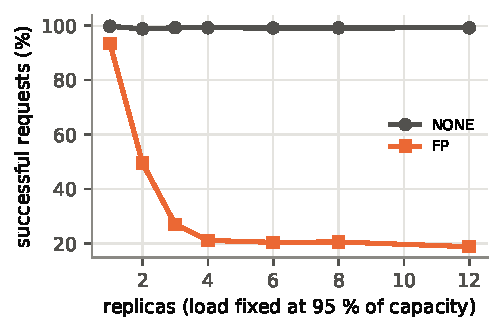
\includegraphics[width=\columnwidth]{figures/sim_N_replicas.pdf}
\caption{Evidence for G1 (simulator, 10 runs per point, 95\,\% load).
With one replica the fast probe does almost no harm. With more replicas
it produces a cascade.}
\label{fig:N}
\end{figure}

\textbf{Research questions for the rest of the project.}
\begin{itemize}
\item \emph{RQ1} (Cutoff~1): under overload, at which probe settings does
  self-healing reduce availability compared with no probe?
\item \emph{RQ2:} can a liveness signal tell slow from dead well enough
  to remove these false restarts while still catching real hangs?
\item \emph{RQ3:} does deciding restarts across replicas prevent
  cascades when the cause is shared?
\end{itemize}

%======================================================================
\section{Proposed Methodology}
\label{sec:method}
%======================================================================
This section is written so that it can move into the final paper with
few changes. Fig.~\ref{fig:arch} gives the overview.

\begin{figure*}[t]
\centering
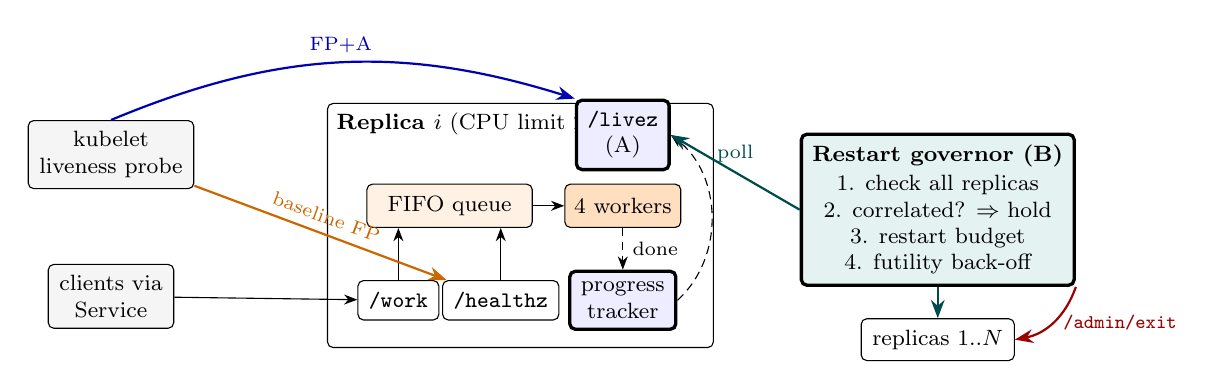
\begin{tikzpicture}[
  font=\footnotesize, >=Stealth,
  box/.style={draw, rounded corners=2pt, align=center, inner sep=4pt},
  pool/.style={draw, fill=orange!10, rounded corners=2pt, minimum width=2.1cm, minimum height=0.55cm},
  comp/.style={draw, very thick, fill=blue!7, rounded corners=2pt, align=center, inner sep=4pt},
  compb/.style={draw, very thick, fill=teal!10, rounded corners=2pt, align=center, inner sep=4pt}]
  % replica
  \node[box, minimum width=4.9cm, minimum height=3.1cm] (rep) at (0,0) {};
  \node[anchor=north west] at (rep.north west) {\textbf{Replica $i$} (CPU limit 200m)};
  \node[pool] (q) at (-0.9,0.25) {FIFO queue};
  \node[pool, fill=orange!25, minimum width=1.2cm] (w) at (1.3,0.25) {4 workers};
  \draw[->] (q) -- (w);
  \node[box, fill=white] (work) at (-1.55,-0.95) {\texttt{/work}};
  \node[box, fill=white] (hz) at (-0.25,-0.95) {\texttt{/healthz}};
  \draw[->] (work) -- (q.south -| work);
  \draw[->] (hz) -- (q.south -| hz);
  \node[comp] (tr) at (1.3,-0.95) {progress\\tracker};
  \draw[->, densely dashed] (w) -- node[right, font=\scriptsize]{done} (tr);
  \node[comp] (lz) at (1.3,1.15) {\texttt{/livez}\\(A)};
  \draw[->, densely dashed] (tr.east) to[bend right=50] (lz.east);
  % kubelet
  \node[box, fill=gray!8] (kl) at (-5.2,0.9) {kubelet\\liveness probe};
  \draw[->, thick, orange!80!black] (kl) -- node[above, font=\scriptsize, sloped]{baseline FP} (hz);
  \draw[->, thick, blue!70!black] (kl.north) to[bend left=20] node[above, font=\scriptsize]{FP+A} (lz.north west);
  \node[box, fill=gray!8] (lb) at (-5.2,-0.9) {clients via\\Service};
  \draw[->] (lb) -- (work);
  % governor
  \node[compb] (gov) at (5.3,0.2) {\textbf{Restart governor (B)}\\[1pt]
     1. check all replicas\\2. correlated? $\Rightarrow$ hold\\3. restart budget\\4. futility back-off};
  \draw[->, thick, teal!60!black] (gov.west) -- node[above, font=\scriptsize]{poll} (lz.east);
  \node[box, minimum width=1.6cm, fill=white] (others) at (5.3,-1.45) {replicas $1..N$};
  \draw[->, thick, teal!60!black] (gov) -- (others);
  \draw[->, thick, red!60!black] (gov.south east) to[bend left=30] node[right, font=\scriptsize]{\texttt{/admin/exit}} (others.east);
\end{tikzpicture}
\caption{Proposed method. Baseline FP probes \texttt{/healthz}, which
waits in the same FIFO queue as real work. Component~A answers
\texttt{/livez} from a progress tracker outside the queue. Component~B
replaces the per-container restart decision with one decision over all
replicas.}
\label{fig:arch}
\end{figure*}

\subsection{Problem definition}
A Deployment has $N$ replicas. Replica $i$ serves requests through a
bounded pool and keeps a queue of pending work $q_i(t)$. A liveness
mechanism is a function that, at each check time $t$, decides whether
to restart replica $i$. We want a mechanism that:
\begin{enumerate}
\item never restarts a replica that is \emph{making progress}, however
  slowly (no false positives under overload);
\item restarts a replica that has \emph{stopped making progress} within
  a bounded time (no false negatives for hangs);
\item does not restart many replicas at once for a cause that a restart
  cannot fix.
\end{enumerate}

\subsection{Component A: progress-based liveness (PBL)}
Each replica keeps two numbers: the count of pending requests $p_i$
(queued or running) and the time $\ell_i$ of the last \emph{completed}
request. The liveness answer is
\begin{equation}
\mathrm{alive}_i(t) \;=\; \big[p_i(t)=0\big] \;\lor\; \big[t-\ell_i(t) < W\big]
\label{eq:pbl}
\end{equation}
where $W$ is the \emph{stall window}. Two details make this robust:
\begin{itemize}
\item When $p_i$ goes from 0 to 1, $\ell_i$ is reset to now. An idle
  container is therefore never ``stalled since the last request an hour
  ago''.
\item Requests that clients abandon while still queued do \emph{not}
  count as progress, so a hung pool cannot look alive just because
  clients keep timing out.
\end{itemize}
The check is served \emph{outside} the worker pool, so it answers in
microseconds whatever the queue length. It is a standard HTTP endpoint
used by an \emph{unmodified} kubelet probe (\texttt{/livez}, FP timing).
It is about 40 lines of Go logic (\texttt{src/internal/progress}) and needs one
\texttt{Begin()} and one \texttt{End()} call around request handling.

Equation~\eqref{eq:pbl} classifies the three cases correctly:
\begin{itemize}
\item an overloaded container keeps completing work, so it is alive;
\item a hung container has $p_i>0$ but completes nothing, so it is dead
  after $W$;
\item an idle container has $p_i=0$, so it is alive.
\end{itemize}
It is the classic heartbeat or watchdog idea from failure-detector
theory~\cite{chandra1996,hayashibara2004}, applied to the container's
\emph{work} instead of to a probe's round-trip time.

\emph{Why not simply isolate the health check?} A health endpoint on its
own thread that always returns 200 (the ISO arm) also avoids false
positives under overload. It can never detect a hang, though, which is
the false-negative problem of Flora \emph{et al.}~\cite{flora2022}. A
keeps hang detection, as the H experiment shows.

\subsection{Component B: cluster-aware restart governor (CRG)}
The governor replaces the kubelet's liveness decision; the Deployment
then has no \texttt{livenessProbe}. Every $P{=}1$\,s it checks every
replica (\texttt{/livez} with A, \texttt{/healthz} without) and applies
Algorithm~\ref{alg:gov}.

\begin{algorithm}[t]
\caption{One governor tick}
\label{alg:gov}
\footnotesize
\begin{algorithmic}[1]
\State $E \gets$ running replicas older than grace $G$ (10\,s)
\State $S \gets \{i\in E : \text{consecutive failed checks}_i \ge F\}$
\If{$S=\emptyset$} \State reset hold; \Return \EndIf
\If{$|S|/N \ge \theta$ \textbf{and} $|S|\ge 2$} \Comment{correlated}
  \If{hold not started} start hold \EndIf
  \If{hold age $< H$} \State emit event \textsc{RestartHeld}; \Return \EndIf
\EndIf
\State $b \gets \max(1,\lfloor \beta N\rfloor) - |\text{in-flight restarts}|$
\State restart up to $b$ replicas of $S$, most failures first
\State \textbf{futility:} if a replica we restarted fails again within
       $R$ (30\,s) of recovering, set $H \gets \min(2H, H_{\max})$
\end{algorithmic}
\end{algorithm}

The three rules each target a failure mode:
\begin{itemize}
\item The \emph{correlation guard} ($\theta{=}0.5$, $H{=}60$\,s) treats
  many replicas failing together as a sign of a shared cause, which a
  restart will not fix.
\item The \emph{budget} ($\beta{=}0.25$) works like
  \texttt{maxUnavailable}: it never takes down more than a quarter of
  the replicas at once.
\item The \emph{futility back-off} lengthens the hold when restarts
  demonstrably do not help.
\end{itemize}
A single hung replica never trips the guard, so it is restarted as soon
as it is a suspect.

The governor restarts a replica \emph{in place} by calling its
\texttt{/admin/exit} hook. The process exits and the kubelet restarts
the container with its normal back-off, so a governor restart costs the
same as a kubelet restart and the comparison is fair. If the hook does
not answer, the governor deletes the pod.

The decision logic is a pure function (\texttt{src/internal/policy}) with
unit tests, and the simulator mirrors it line by line. The controller
is a 1-replica Deployment. Together with the policy it is about 400
lines and uses only the Go standard library.

\subsection{How the components map to the gap}
\begin{itemize}
\item A answers G2 (slow vs.\ dead) without asking the application to
  log its own failure, which SKI does require.
\item B answers G3 (no aggregation), which is a limitation the paper
  names itself.
\item Testing with $N=6$ replicas, under load and with three kinds of
  stress answers G1.
\end{itemize}

\subsection{Parameters and their trade-off}
$W$ is the only important parameter of A. A small $W$ catches hangs
fast but treats short stalls as hangs. Detection time is about $W+P$
(Sec.~\ref{sec:sens}). We use $W{=}5$\,s, which is 100 times the normal
service time. B's parameters behave like rolling-update settings, and
the results are not sensitive to $\theta$ (Table~\ref{tab:G}).

\subsection{Overhead}
A needs two atomic counters per request. B adds one pod and $N$ small
HTTP checks per second. On the testbed the governor used
\TBN{govcpu}\,CPU-seconds and \TBN{govmib}\,MiB per run.

%======================================================================
\section{Experimental Design}
\label{sec:design}
%======================================================================
\subsection{Arms}
Every arm uses the same service, readiness probe, replicas and load;
only the liveness mechanism changes.
\begin{itemize}
\item \textbf{NONE}: no liveness probe (control, from Cutoff~1).
\item \textbf{DP}: the paper's default probe timing (3\,s, 3 failures).
\item \textbf{FP}: the paper's fast probe on \texttt{/healthz}
  (1\,s, 1 failure). This is our \textbf{baseline}.
\item \textbf{ISO}: FP timing on an isolated always-200 endpoint.
\item \textbf{\FPA}: FP timing on \texttt{/livez} (Component A).
\item \textbf{\FPB}: governor on \texttt{/healthz} (Component B).
\item \textbf{\FPAB}: governor on \texttt{/livez} (proposed method).
\end{itemize}
The four arms FP, \FPA, \FPB{} and \FPAB{} form the 2$\times$2 ablation
the instructor asked for.

\subsection{Scenarios}
\begin{itemize}
\item \textbf{R}: the paper's reproduction (Sec.~\ref{sec:reproresults}).
\item \textbf{C}: calibration; measures the capacity of one replica and
  how probe latency grows with load.
\item \textbf{O}: sustained load (no fault) at 50--150\,\% of capacity.
\item \textbf{P}: a 60\,s spike from 70\,\% to 150\,\%, then back to
  70\,\%.
\item \textbf{H}: one replica hangs silently at 60\,s (a real failure
  that must be caught).
\item \textbf{D}: the shared dependency stalls for 20\,s (every replica
  stops at once; a restart cannot help).
\item \textbf{S}: the Cutoff-1 grid of timeoutSeconds $\{1,2,5\}$
  $\times$ failureThreshold $\{1,3,10\}$ at period 5\,s.
\end{itemize}

\subsection{Metrics}
\begin{itemize}
\item \textbf{Success rate}: requests answered with 2xx within the 2\,s
  client timeout.
\item \textbf{Restarts}: container restarts during the load window.
\item \textbf{Availability}: mean fraction of Ready replicas.
\item \textbf{Cascade depth}: the largest number of replicas not Ready
  at the same time.
\item \textbf{Post-spike success} (P): success rate after the spike ends.
\item \textbf{Recovery time} (P, D): seconds from the end of the stress
  until per-second success stays $\ge 90\,\%$ for 5\,s.
\item \textbf{Detection time} (H): time from fault to the restart
  decision.
\item \textbf{p95/p99 latency} of successful requests.
\item \textbf{Overhead}: CPU and memory used.
\end{itemize}

\subsection{Statistics}
The simulator runs 10--30 seeds per cell. We report means and, where
useful, standard deviations. Testbed cells have 1--5 repetitions, which
is enough to confirm the direction and size of effects that the
simulator shows clearly. Arms are interleaved, so slow drift of the
machine affects all arms equally.

%======================================================================
\section{Results}
\label{sec:results}
%======================================================================
Unless stated otherwise, all numbers are means over seeds. ``Sim'' means
simulator and ``TB'' means Kubernetes testbed.

\subsection{Calibration: load turns into probe latency (C)}
Before using Kubernetes we checked the coupling on \emph{real processes}
with \texttt{experiments/local\_check.py}. One SUT process ran pinned to
one core (\locMode), and our load generator measured it. The measured
capacity was \locCap\,req/s.
\begin{itemize}
\item At 50\,\% load, \texttt{/healthz} answered in \locHzFifty\,ms and
  \texttt{/livez} in \locLzFifty\,ms (medians).
\item At 90\,\% load, \texttt{/healthz} rose to \locHzNinety\,ms, while
  \texttt{/livez} stayed at \locLzNinety\,ms.
\item At 150\,\% load, \locHzFailOneFifty{} \texttt{/healthz} checks hit
  the 1\,s probe timeout. \texttt{/livez} still answered in
  \locLzOneFifty\,ms.
\item After a silent hang, \texttt{/livez} switched to 503 after
  \locHang\,s ($=W$), as designed. The isolated check (ISO) never failed.
\end{itemize}
This is the gap mechanism in miniature. The baseline check fails
because of load alone, while Component~A does not.

One practical lesson came out of this test. If the Go runtime has only
one scheduler thread (\texttt{GOMAXPROCS=1}), a saturated process
delays even \texttt{/livez} beyond 1\,s. In that case A would also give
false positives. In a pod, Go~1.22 uses the host CPU count (8 on the
HP~348), so the problem does not arise, but deployments must keep
\texttt{GOMAXPROCS} above the pool size
(\texttt{results/local/local\_check\_gomaxprocs1.json}).

On the testbed, the measured capacity of one replica with a 200m limit
is \TBN{cap}\,req/s (Table~\ref{tab:C}, Fig.~\ref{fig:C}).

\IfFileExists{generated/tb_table_C.tex}{%
\begin{table}[t]
\centering
\caption{TB calibration: one replica, no liveness probe}
\label{tab:C}
\footnotesize
\begin{tabular}{@{}rrrrrrr@{}}
\toprule
Rate & Goodput & Succ. & p95 & \multicolumn{2}{c}{\texttt{/healthz} ms} & \texttt{/livez} \\
req/s & req/s & \% & ms & median & max & ms \\
\midrule
\tabinput{generated/tb_table_C.tex}
\bottomrule
\end{tabular}
\end{table}
\begin{figure}[t]
\centering
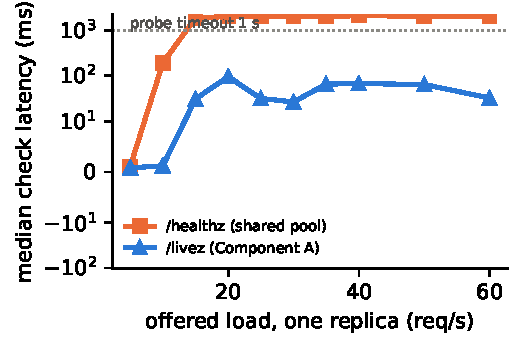
\includegraphics[width=0.9\columnwidth]{figures/tb_C_coupling.pdf}
\caption{TB: health-check latency against load for one replica.}
\label{fig:C}
\end{figure}}{%
\begin{table}[t]\centering\caption{TB calibration}\label{tab:C}\footnotesize
\begin{tabular}{c}\toprule \textit{pending -- run \texttt{experiments/02\_calibrate.sh}}\\ \bottomrule\end{tabular}\end{table}
\begin{figure}[t]\centering\fbox{\parbox{0.9\columnwidth}{\centering\footnotesize Figure appears after the testbed run.}}
\caption{TB: health-check latency against load.}\label{fig:C}\end{figure}}

\subsection{Sustained load: probes manufacture failures (O)}
Fig.~\ref{fig:O} and Table~\ref{tab:O} answer RQ1 and RQ2.
\begin{itemize}
\item \textbf{Up to 80\,\% load}, all arms behave the same.
\item \textbf{At 90\,\% load}, nothing is broken: NONE serves
  \simOnineNONEsucc\,\% of requests. FP restarts containers
  \simOnineFPrestarts{} times, Ready replicas drop to
  \simOnineFPavail\,\% and success falls to \simOnineFPsucc\,\%.
\item \textbf{At 100\,\% load}, FP gives \simOhundredFPsucc\,\% success
  and DP gives \simOhundredDPsucc\,\%, against \simOhundredNONEsucc\,\%
  with no probe. \emph{No liveness probe is strictly better than a
  standard one}, which was the headline we expected in Cutoff~1.
\item \textbf{Component A} removes every false restart at every load:
  \FPA{} matches NONE.
\item \textbf{Component B alone} reduces the damage
  (\simOhundredBrestarts{} restarts and \simOhundredBsucc\,\% success at
  100\,\%) but does not remove it. Its check is still the queued
  \texttt{/healthz}, and when the hold expires the budgeted restarts
  resume.
\end{itemize}

\begin{figure*}[t]
\centering
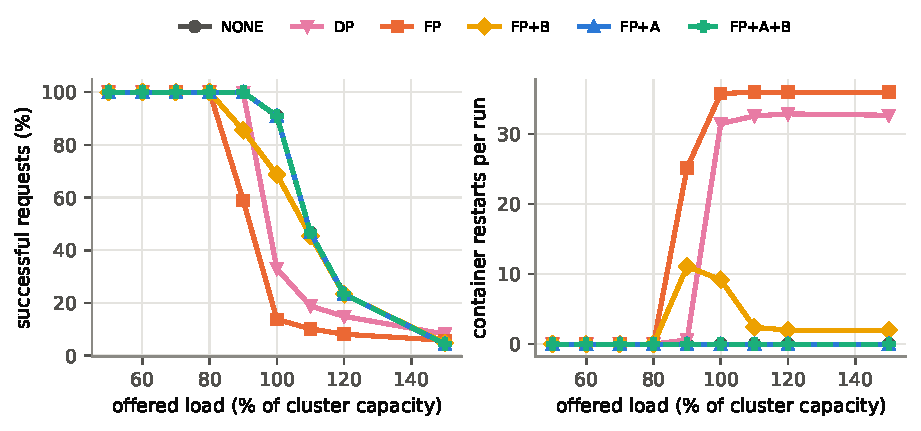
\includegraphics[width=0.9\textwidth]{figures/sim_O_load.pdf}
\caption{Sim, sustained load (10 runs per point). Left: success rate.
Right: restarts per 240\,s run. FP and DP restart healthy containers
from 90\,\% load. Component A (and A+B) removes every one of these
false restarts.}
\label{fig:O}
\end{figure*}

\begin{table*}[t]
\centering
\caption{Sustained load (O): success rate (\%) and restarts per run}
\label{tab:O}
\footnotesize
\begin{tabular}{@{}lcccccccc@{}}
\toprule
& \multicolumn{2}{c}{60\,\%} & \multicolumn{2}{c}{90\,\%} & \multicolumn{2}{c}{100\,\%} & \multicolumn{2}{c}{120\,\%} \\
\cmidrule(lr){2-3}\cmidrule(lr){4-5}\cmidrule(lr){6-7}\cmidrule(lr){8-9}
Arm (Sim) & Succ. & Restarts & Succ. & Restarts & Succ. & Restarts & Succ. & Restarts \\
\midrule
\tabinput{generated/sim_table_O.tex}
\bottomrule
\end{tabular}

\vspace{4pt}
\IfFileExists{generated/tb_table_O.tex}{%
\begin{tabular}{@{}lcccc@{}}
\toprule
Arm (TB, load \TBN{Oloads}) & Succ.\,\% & Restarts & Ready\,\% & p99 ms \\
\midrule
\tabinput{generated/tb_table_O.tex}
\bottomrule
\end{tabular}}{\footnotesize\textit{Testbed rows (90\,\% load) appear here after \texttt{experiments/03\_overload.sh}.}}
\end{table*}

\subsection{A short spike becomes a lasting outage (P)}
Fig.~\ref{fig:P} and Table~\ref{tab:P} show the most striking result.
During the 60\,s spike every arm drops requests, because the capacity is
simply not there. When the load returns to 70\,\%, NONE recovers in
about 2\,s.

FP does \emph{not} recover. Replicas restarted during the spike sit in
CrashLoopBackOff, the survivors are overloaded, fail their probes and
are restarted in turn. The service stays at \simPFPpost\,\% success for
the remaining two minutes, long after the trigger is gone. This is a
\emph{metastable failure}~\cite{bronson2021,huang2022} caused by the
self-healing loop itself. DP recovers after about \simPDPrec\,s. \FPA{}
and \FPAB{} recover like NONE (\simPABpost\,\%).

\begin{figure*}[t]
\centering
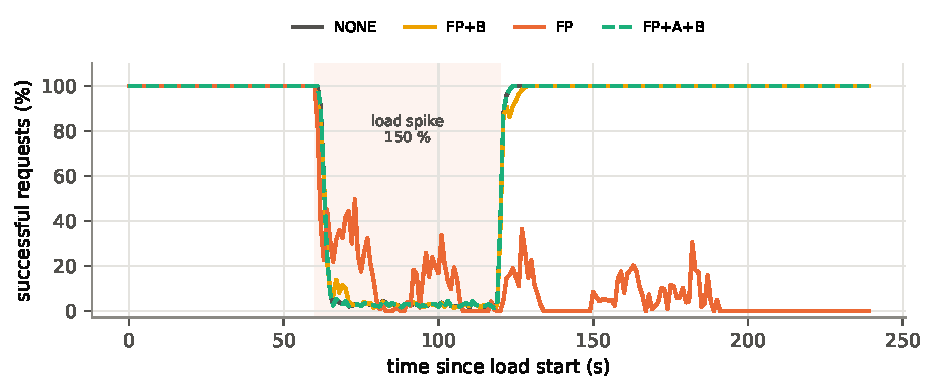
\includegraphics[width=0.9\textwidth]{figures/sim_P_timeline.pdf}
\caption{Sim, load spike (mean of 10 runs). After the spike, FP stays
down: the probe loop keeps the system in a bad state (metastable
failure). The proposed A+B recovers at once.}
\label{fig:P}
\end{figure*}

\begin{table}[t]
\centering
\caption{Load spike to 150\,\% (P)}
\label{tab:P}
\footnotesize
\begin{tabular}{@{}lcccc@{}}
\toprule
Arm & Restarts & Ready\,\% & Post-spike succ.\,\% & Recovery s \\
\midrule
\multicolumn{5}{@{}l}{\textit{Simulator (10 runs)}}\\
\tabinput{generated/sim_table_P.tex}
\midrule
\multicolumn{5}{@{}l}{\textit{Testbed}}\\
\tbrows{P}
\bottomrule
\end{tabular}
\end{table}

\subsection{Real hangs are still caught (H)}
A method that never restarts anything would ``win'' every overload test.
Experiment~H checks that real hangs are still caught. One replica hangs
silently at 60\,s (Table~\ref{tab:H}).
\begin{itemize}
\item NONE and ISO \emph{never} detect the hang. That replica stays
  useless and capacity is lost for good, which is the false-negative
  problem.
\item SKI would behave like NONE, because a hung process writes no log
  line.
\item FP and \FPB{} detect the hang in \simHFPdet\,s.
\item \FPA{} and \FPAB{} detect it in \simHABdet\,s, roughly $W$.
\end{itemize}
This is the price of A: about 4\,s slower detection, which buys immunity
to overload. Success rates for all detecting arms stay above 99\,\%.

\begin{table}[t]
\centering
\caption{Silent hang of one replica (H, 70\,\% load)}
\label{tab:H}
\footnotesize
\begin{tabular}{@{}lcccc@{}}
\toprule
Arm & Detected & Detect.\ time s & Success & Ready\,\% \\
\midrule
\multicolumn{5}{@{}l}{\textit{Simulator (20 runs)}}\\
\tabinput{generated/sim_table_H.tex}
\midrule
\multicolumn{5}{@{}l}{\textit{Testbed}}\\
\tbrows{H}
\bottomrule
\end{tabular}
\end{table}

\subsection{Shared brown-out: why B is needed (D)}
In a dependency stall every replica stops completing work at the same
time, so no single container is at fault. Here Component~A alone is
\emph{not} enough. After $W$ seconds without progress, every replica
looks hung, and \FPA{} restarts \simDArestarts{} containers per run.
FP is worse still, with \simDFPrestarts{} restarts and
\simDFPsucc\,\% success.

The governor's correlation guard sees that six of six replicas fail
together and holds the restarts. \FPAB{} makes \simDABrestarts{}
restarts and reaches \simDABsucc\,\% success, which equals NONE
(\simDNONEsucc\,\%), the best possible result for a 20\,s outage
(Fig.~\ref{fig:D}, Table~\ref{tab:D}).

\begin{figure*}[t]
\centering
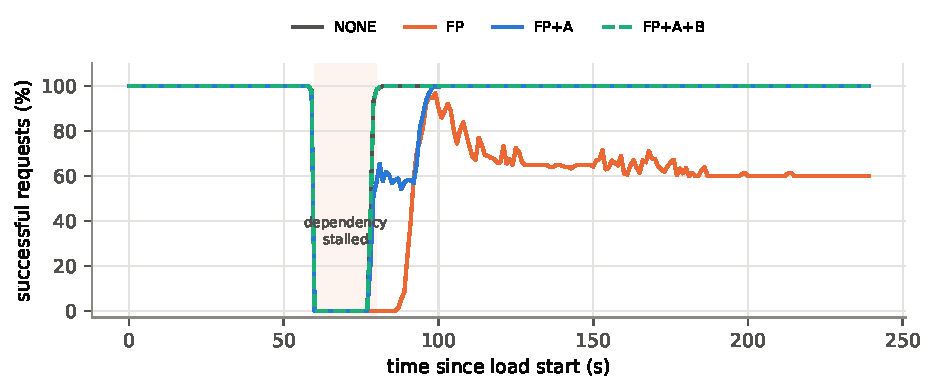
\includegraphics[width=0.9\textwidth]{figures/sim_D_timeline.pdf}
\caption{Sim, 20\,s dependency stall (mean of 20 runs). A alone
restarts every replica once progress has stopped for $W$\,s. Only A+B
recovers like NONE as soon as the dependency returns.}
\label{fig:D}
\end{figure*}

\begin{table}[t]
\centering
\caption{Dependency stall of 20\,s (D, 70\,\% load)}
\label{tab:D}
\footnotesize
\begin{tabular}{@{}lcccc@{}}
\toprule
Arm & Restarts & Success & Bad s & Recovery s \\
\midrule
\multicolumn{5}{@{}l}{\textit{Simulator (20 runs)}}\\
\tabinput{generated/sim_table_D.tex}
\midrule
\multicolumn{5}{@{}l}{\textit{Testbed}}\\
\tbrows{D}
\bottomrule
\end{tabular}

\vspace{2pt}\raggedright\footnotesize
``Bad s'' = seconds with less than 50\,\% successful requests (20 are
unavoidable). Recovery is measured from the end of the stall; ``(k/n)''
means only k of n runs recovered within the run.
\end{table}

\subsection{Ablation}
Table~\ref{tab:ablation} isolates each component.
\begin{itemize}
\item \textbf{A alone} fixes overload (O, P) but not shared stalls (D).
\item \textbf{B alone} fixes shared stalls and most of the spike, but
  still restarts under sustained 90\,\% load.
\item \textbf{A+B} is the only combination that is best or tied-best in
  every column except hang-detection speed, where it pays the expected
  $\approx W$.
\end{itemize}
Each component is therefore responsible for a different part of the
improvement.

\begin{table*}[t]
\centering
\caption{Ablation over the four stress scenarios (higher success is
better; fewer restarts and faster detection are better)}
\label{tab:ablation}
\footnotesize
\begin{tabular}{@{}lcccccccc@{}}
\toprule
& & & \multicolumn{2}{c}{O: 90\,\% load} & P: spike & H: hang & \multicolumn{2}{c}{D: dependency stall} \\
\cmidrule(lr){4-5}\cmidrule(lr){6-6}\cmidrule(lr){7-7}\cmidrule(lr){8-9}
System & A & B & Succ.\,\% & Restarts & Post-spike succ.\,\% & Detect.\ s & Restarts & Succ.\,\% \\
\midrule
\multicolumn{9}{@{}l}{\textit{Simulator}}\\
\tabinput{generated/sim_table_ablation.tex}
\midrule
\multicolumn{9}{@{}l}{\textit{Testbed}}\\
\tbrows{ablation}
\bottomrule
\end{tabular}
\end{table*}

\subsection{Where is the boundary? (Cutoff-1 RQ1, S)}
\label{sec:sweep}
Fig.~\ref{fig:S} sweeps the Cutoff-1 grid with \texttt{periodSeconds}=5.
The probe causes harm (more than 1 point below the control) in
\simSharmful{} of 27 cells, and all of them are at 100\,\% load. Large
harm (44--72 points) occurs only with \texttt{timeoutSeconds}=1 and
\texttt{failureThreshold}$\le 3$. A 2\,s timeout or a threshold of 10
cuts the harm to a few points at this load.

At 50\,\% load the probe is harmless. At 150\,\% load the control has
already collapsed, and restarts even help a little, because killing a
container empties its queue of requests that are already doomed. The
boundary is therefore a \emph{band} around saturation, and it is
narrower with a slow period (5\,s) than with FP (1\,s), where harm starts
at 90\,\% (Fig.~\ref{fig:O}).

\begin{figure*}[t]
\centering
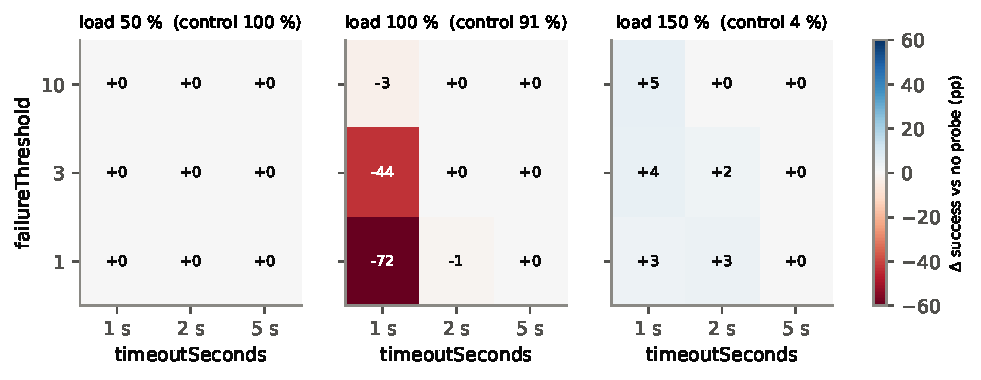
\includegraphics[width=0.9\textwidth]{figures/sim_S_heatmap.pdf}
\caption{Sim, Cutoff-1 sweep (period 5\,s, 10 runs per cell): change in
success rate against no probe, in percentage points. Red = the probe
made things worse.}
\label{fig:S}
\end{figure*}

\subsection{Sensitivity}
\label{sec:sens}
\textbf{Stall window $W$} (Table~\ref{tab:W}, Fig.~\ref{fig:W}).
Detection time grows as $W+0.3$\,s. False restarts during a 20\,s stall
fall only once $W$ approaches the stall length. No single $W$ handles
both hangs and long brown-outs, and this is exactly why B is needed:
with B, $W$ can stay small.

Overload never causes false restarts with A, whatever the value of $W$,
because an overloaded replica always makes progress.

\textbf{Governor} (Table~\ref{tab:G}). With 6 of 6 replicas stalled,
any $\theta\le0.67$ holds the restarts. A hold shorter than the stall
(30\,s against a 40\,s stall) lets one budgeted restart through. Turning
the guard off (budget only) gives 8 restarts.

\begin{table}[t]
\centering
\caption{Sim: effect of the stall window $W$ (A only)}
\label{tab:W}
\footnotesize
\begin{tabular}{@{}rccc@{}}
\toprule
$W$ (s) & H: detect.\ s & D: restarts & O 100\,\%: restarts \\
\midrule
\tabinput{generated/sim_table_W.tex}
\bottomrule
\end{tabular}
\end{table}

\begin{figure}[t]
\centering
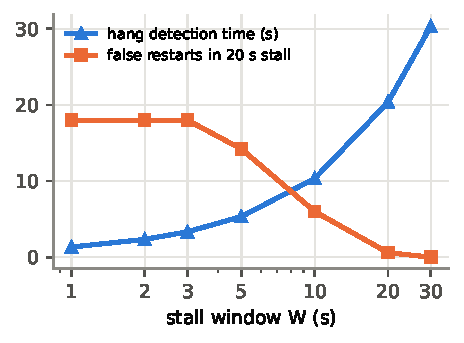
\includegraphics[width=0.9\columnwidth]{figures/sim_W_tradeoff.pdf}
\caption{Sim: the $W$ trade-off for Component A alone.}
\label{fig:W}
\end{figure}

\begin{table}[t]
\centering
\caption{Sim: governor parameters (A+B, 40\,s stall / hang)}
\label{tab:G}
\footnotesize
\begin{tabular}{@{}cccccc@{}}
\toprule
$\theta$ & $H$ (s) & D: restarts & D: succ.\,\% & H: detect.\ s \\
\midrule
\tabinput{generated/sim_table_G.tex}
\bottomrule
\end{tabular}
\end{table}

%======================================================================
\section{Final Comparison and Discussion}
\label{sec:final}
%======================================================================
Table~\ref{tab:final} brings everything together.

\begin{table*}[t]
\centering
\caption{Final comparison: original paper, reproduced baseline and
proposed method}
\label{tab:final}
\footnotesize
\begin{tabular}{@{}p{4.6cm}p{3.1cm}p{3.6cm}p{4.2cm}@{}}
\toprule
& Original paper~\cite{roberts2025} & Reproduced baseline (FP) & Proposed (FP+A+B) \\
\midrule
Setting & 1 pod, $\le$100\,req/s & 1 pod (R) and 6 pods (O, P, H, D) & 6 pods \\
Process crash: time to queue restart & 0.7\,s (FP), 0.1\,s (SKI) & 0.8\,s (sim) / \TB{FP}{q}\,s (TB) & not re-measured (a dead process refuses the connection, so the check fails at once) \\
Silent hang: detection & not tested & \simHFPdet\,s & \simHABdet\,s ($\approx W$) \\
90\,\% load, no fault: success & not tested & \simOnineFPsucc\,\% (\simOnineFPrestarts{} restarts) & 100\,\% (0 restarts) \\
After 60\,s spike: success & not tested & \simPFPpost\,\% & \simPABpost\,\% \\
20\,s dependency stall: success & not tested & \simDFPsucc\,\% & \simDABsucc\,\% \\
Extra runtime cost & SKI: +0.04 vCPU, +9\,MiB per pod & -- & 2 counters/request; 1 governor pod (\TBN{govmib}\,MiB) \\
Needs modified kubelet? & Yes & No & No \\
Needs app to log its failure? & Yes (SKI) & No & No (needs \texttt{Begin/End} hooks) \\
\bottomrule
\end{tabular}
\end{table*}

\textbf{What was reproduced?} The detection-time model and the
DP/FP/SKI detection times, within about 1\,s. The ranking and size of the
availability differences. The FP extra-restart anomaly, which we also
explain.

\textbf{What could not be reproduced?} SKI's exact mechanism, because
the modified kubelet is not public; we reproduce its behaviour instead.
The paper's total and failed request counts, which depend on undocumented
Locust settings. The ``catalogue bug''. And 30 repetitions on real
hardware, where we run 3--5.

\textbf{Why are there differences?} The client model, container runtime,
hardware, start-up time and the paper's own one-second model error
(Sec.~\ref{sec:diff}).

\textbf{What gap was identified?} Monitoring that confuses slow with
dead and decides per container, which a single-pod evaluation cannot
expose (Sec.~\ref{sec:gap}).

\textbf{How does the proposal address it?} A judges progress, not
latency. B decides across replicas.

\textbf{What is the evidence?} The 2$\times$2 ablation over four stress
scenarios (Table~\ref{tab:ablation}); the replica-count experiment
(Fig.~\ref{fig:N}); and real-process measurements of the
latency--load coupling. Testbed confirmation is in the TB rows.

\textbf{Remaining limitations.} A needs two hooks in the application,
and its check needs a free scheduler thread (\texttt{GOMAXPROCS} above
the pool size).
This is a smaller change than SKI's log contract, but it is still a
change. Detection of silent hangs is slower by about $W$. If many
replicas hang at the \emph{same} time from a bug inside each pod, B
delays the needed restarts by up to $H$. The futility rule and the hold
bound this delay, but do not remove it.

%======================================================================
\section{Threats to Validity}
\label{sec:threats}
%======================================================================
\textbf{Simulation is a model.} Processor sharing ignores the 100\,ms CFS
quota periods. The simulator also assumes that \texttt{/livez} answers
instantly; the real-process check shows this holds only when the
runtime has spare scheduler threads. Endpoint and back-off timing are simplified from the
Kubernetes source. We reduce this threat in three ways: by reproducing
the paper's numbers first, by checking the coupling on real processes,
and by running every scenario on the real testbed.

\textbf{Single host.} CPU limits make each pod saturate before the
laptop does. The calibration reports the \emph{measured} capacity.

\textbf{Synthetic service.} Our SUT is minimal on purpose. The mechanism
that generalises is a health check that shares resources with work.
\texttt{catalogue}'s \texttt{/health} has the same property through its
database.

\textbf{Few testbed repetitions.} Effects of tens of percentage points
are visible in 1--5 runs. Small differences are judged only on the
simulator.

%======================================================================
\section{Points for Mentor Discussion and Next Steps}
%======================================================================
\begin{enumerate}
\item Is reproducing SKI's behaviour on stock Kubernetes acceptable,
  given that the authors' modified kubelet is private?
\item Is the gap (G1--G3) accepted as the direction for Cutoff~3?
\item For Cutoff~3 we plan to:
  \begin{itemize}
  \item run the \emph{full} testbed profile;
  \item add a multi-service benchmark (TeaStore or the full SockShop);
  \item add \texttt{catalogue} under load as a second, unmodified
    application;
  \item compare against an adaptive timeout (a $\varphi$-accrual-style
    detector~\cite{hayashibara2004}).
  \end{itemize}
\end{enumerate}

%======================================================================
\section{Conclusion}
%======================================================================
We re-implemented the core of Roberts \emph{et al.} on stock Kubernetes
and in a calibrated simulator, and reproduced its detection times. We
also explained its unexplained restarts.

The reproduction exposed a gap. The paper's single-pod, light-load
setting hides the fact that poll-based self-healing \emph{creates}
outages in replicated services under load. Signal-based monitoring
fixes only part of this.

Our method has two parts. Progress-based liveness tells slow from dead.
A cluster-aware governor refuses to restart replicas that fail together.
Together they remove every false restart in our overload, spike and
brown-out scenarios, and they still catch real hangs.

%======================================================================
\appendices
\section{How to Reproduce Everything}
\label{app:run}
\footnotesize
\begin{verbatim}
# simulator (any laptop, ~5 min, no Docker needed)
python3 sim/run_all.py
# Kubernetes testbed (~5 h, see docs/GUIDE.md)
PROFILE=quick bash experiments/run_all.sh
python3 analysis/analyze_testbed.py
# rebuild this PDF (testbed tables fill in)
cd report && latexmk -pdf main.tex
\end{verbatim}
Repository layout: \texttt{src/} (Go: SUT, load generator, SKI
emulation, governor), \texttt{manifests/}, \texttt{cluster/},
\texttt{experiments/}, \texttt{sim/}, \texttt{analysis/},
\texttt{results/}, \texttt{report/}, \texttt{docs/}.

\normalsize
\bibliographystyle{IEEEtran}
\bibliography{references}

\end{document}
